\documentclass{article}
\usepackage[utf8]{inputenc}
\usepackage{amsmath}
\usepackage{amssymb}
\usepackage[makeroom]{cancel}
\usepackage{tabularx}
\usepackage{arydshln}
\usepackage{graphicx}

\setlength{\parskip}{1em}
\setlength\parindent{0px}
\title{Homework 3}
\date{\today}
\author{John J Li}

\begin{document}
    \pagenumbering{gobble}
    \maketitle
    \newpage
    \pagenumbering{arabic}

    %###################################################################################

    \textbf{Problem 1:}

    % \begin{center}
    %     \begin{tabular} {cccc|c}
    %         A & B & C & D & F \\
    %         \hline
    %         0 & 0 & 0 & 0 & 0 \\
    %         0 & 0 & 0 & 1 & 0 \\
    %         0 & 0 & 1 & 0 & 0 \\
    %         0 & 0 & 1 & 1 & 0 \\
    %         0 & 1 & 0 & 0 & 0 \\
    %         0 & 1 & 0 & 1 & 0 \\
    %         0 & 1 & 1 & 0 & 0 \\
    %         0 & 1 & 1 & 1 & 0 \\
    %         1 & 0 & 0 & 0 & 0 \\
    %         1 & 0 & 0 & 1 & 0 \\
    %         1 & 0 & 1 & 0 & 0 \\
    %         1 & 0 & 1 & 1 & 0 \\
    %         1 & 1 & 0 & 0 & 0 \\
    %         1 & 1 & 0 & 1 & 0 \\
    %         1 & 1 & 1 & 0 & 0 \\
    %         1 & 1 & 1 & 1 & 0 \\
    %     \end{tabular}
    % \end{center}

    \begin{center}
        \begin{tabular} {cccc|c}
            w & x & y & z & f \\
            \hline
            0 & 0 & 0 & 0 & 1 \\
            0 & 0 & 0 & 1 & 1 \\
            0 & 0 & 1 & 0 & 0 \\
            0 & 0 & 1 & 1 & 0 \\
            0 & 1 & 0 & 0 & 0 \\
            0 & 1 & 0 & 1 & 1 \\
            0 & 1 & 1 & 0 & 0 \\
            0 & 1 & 1 & 1 & 1 \\
            1 & 0 & 0 & 0 & 1 \\
            1 & 0 & 0 & 1 & 0 \\
            1 & 0 & 1 & 0 & 1 \\
            1 & 0 & 1 & 1 & 0 \\
            1 & 1 & 0 & 0 & 0 \\
            1 & 1 & 0 & 1 & 1 \\
            1 & 1 & 1 & 0 & 1 \\
            1 & 1 & 1 & 1 & 1 \\
        \end{tabular}
    \end{center}

    \boxed{f(w,x,y,z)=\sum m(0,1,5,7,8,10,13,14,15)}

    %###################################################################################

    \textbf{Problem 2:}

    \quad\quad (i)

    \quad\quad\quad F(a,b,c)
    \begin{center}
        \begin{tabular} {ccc|c|c|c} 
            a & b & c & (ab)' & (b+(ac)') & F(a,b,c) \\
            \hline
            0 & 0 & 0 & 1 & 1 & 1 \\
            0 & 0 & 1 & 1 & 1 & 1 \\
            0 & 1 & 0 & 1 & 1 & 1 \\
            0 & 1 & 1 & 1 & 1 & 1 \\
            1 & 0 & 0 & 1 & 1 & 1 \\
            1 & 0 & 1 & 1 & 0 & 1 \\
            1 & 1 & 0 & 0 & 1 & 1 \\
            1 & 1 & 1 & 0 & 1 & 1 \\
        \end{tabular}
    \end{center}
    \quad\quad\quad G(a,b,c)
    \begin{center}
        \begin{tabular} {ccc|c|c|c} 
            a & b & c & b+a'bc' & (b+c)' & G(a,b,c) \\
            \hline
            0 & 0 & 0 & 1 & 1 & 1 \\
            0 & 0 & 1 & 1 & 0 & 1 \\
            0 & 1 & 0 & 1 & 0 & 1 \\
            0 & 1 & 1 & 0 & 0 & 0 \\
            1 & 0 & 0 & 1 & 1 & 1 \\
            1 & 0 & 1 & 1 & 0 & 1 \\
            1 & 1 & 0 & 0 & 0 & 0 \\
            1 & 1 & 1 & 0 & 0 & 0 \\
        \end{tabular}
    \end{center}

    \quad\quad (ii)

    \quad\quad\quad F(a,b,c)

    \begin{center}
        \begin{tabular} {cc|cccc}
            & bc & &&& \\
            a && 00 & 01 & 11 & 10 \\
            \hline
            & 0 & 1 & 1 & 1 & 1 \\
            & 1 & 1 & 1 & 1 & 1 \\
        \end{tabular}
    \end{center}

    \quad\quad\quad\quad 000/001/011/010/100/101/111/110 rectangle - a,b, and c changed.

    \quad\quad\quad\quad \boxed{F(a,b,c)=1}

    \quad\quad\quad G(a,b,c)

    \begin{center}
        \begin{tabular} {cc|cccc}
            & bc & &&& \\
            a && 00 & 01 & 11 & 10 \\
            \hline
            & 0 & 1 & 1 & 1 & 1 \\
            & 1 & 1 & 0 & 0 & 1 \\
        \end{tabular}
    \end{center}

    \quad\quad\quad\quad 000/001/011/010 row - b and c changed.

    \quad\quad\quad\quad\quad $= a'$

    \quad\quad\quad\quad 100/110 pair - b changed.

    \quad\quad\quad\quad\quad $= ac'$

    \quad\quad\quad\quad \boxed{G(a,b,c) = a' + ac'}

    \quad\quad (iii)

    \begin{center}
        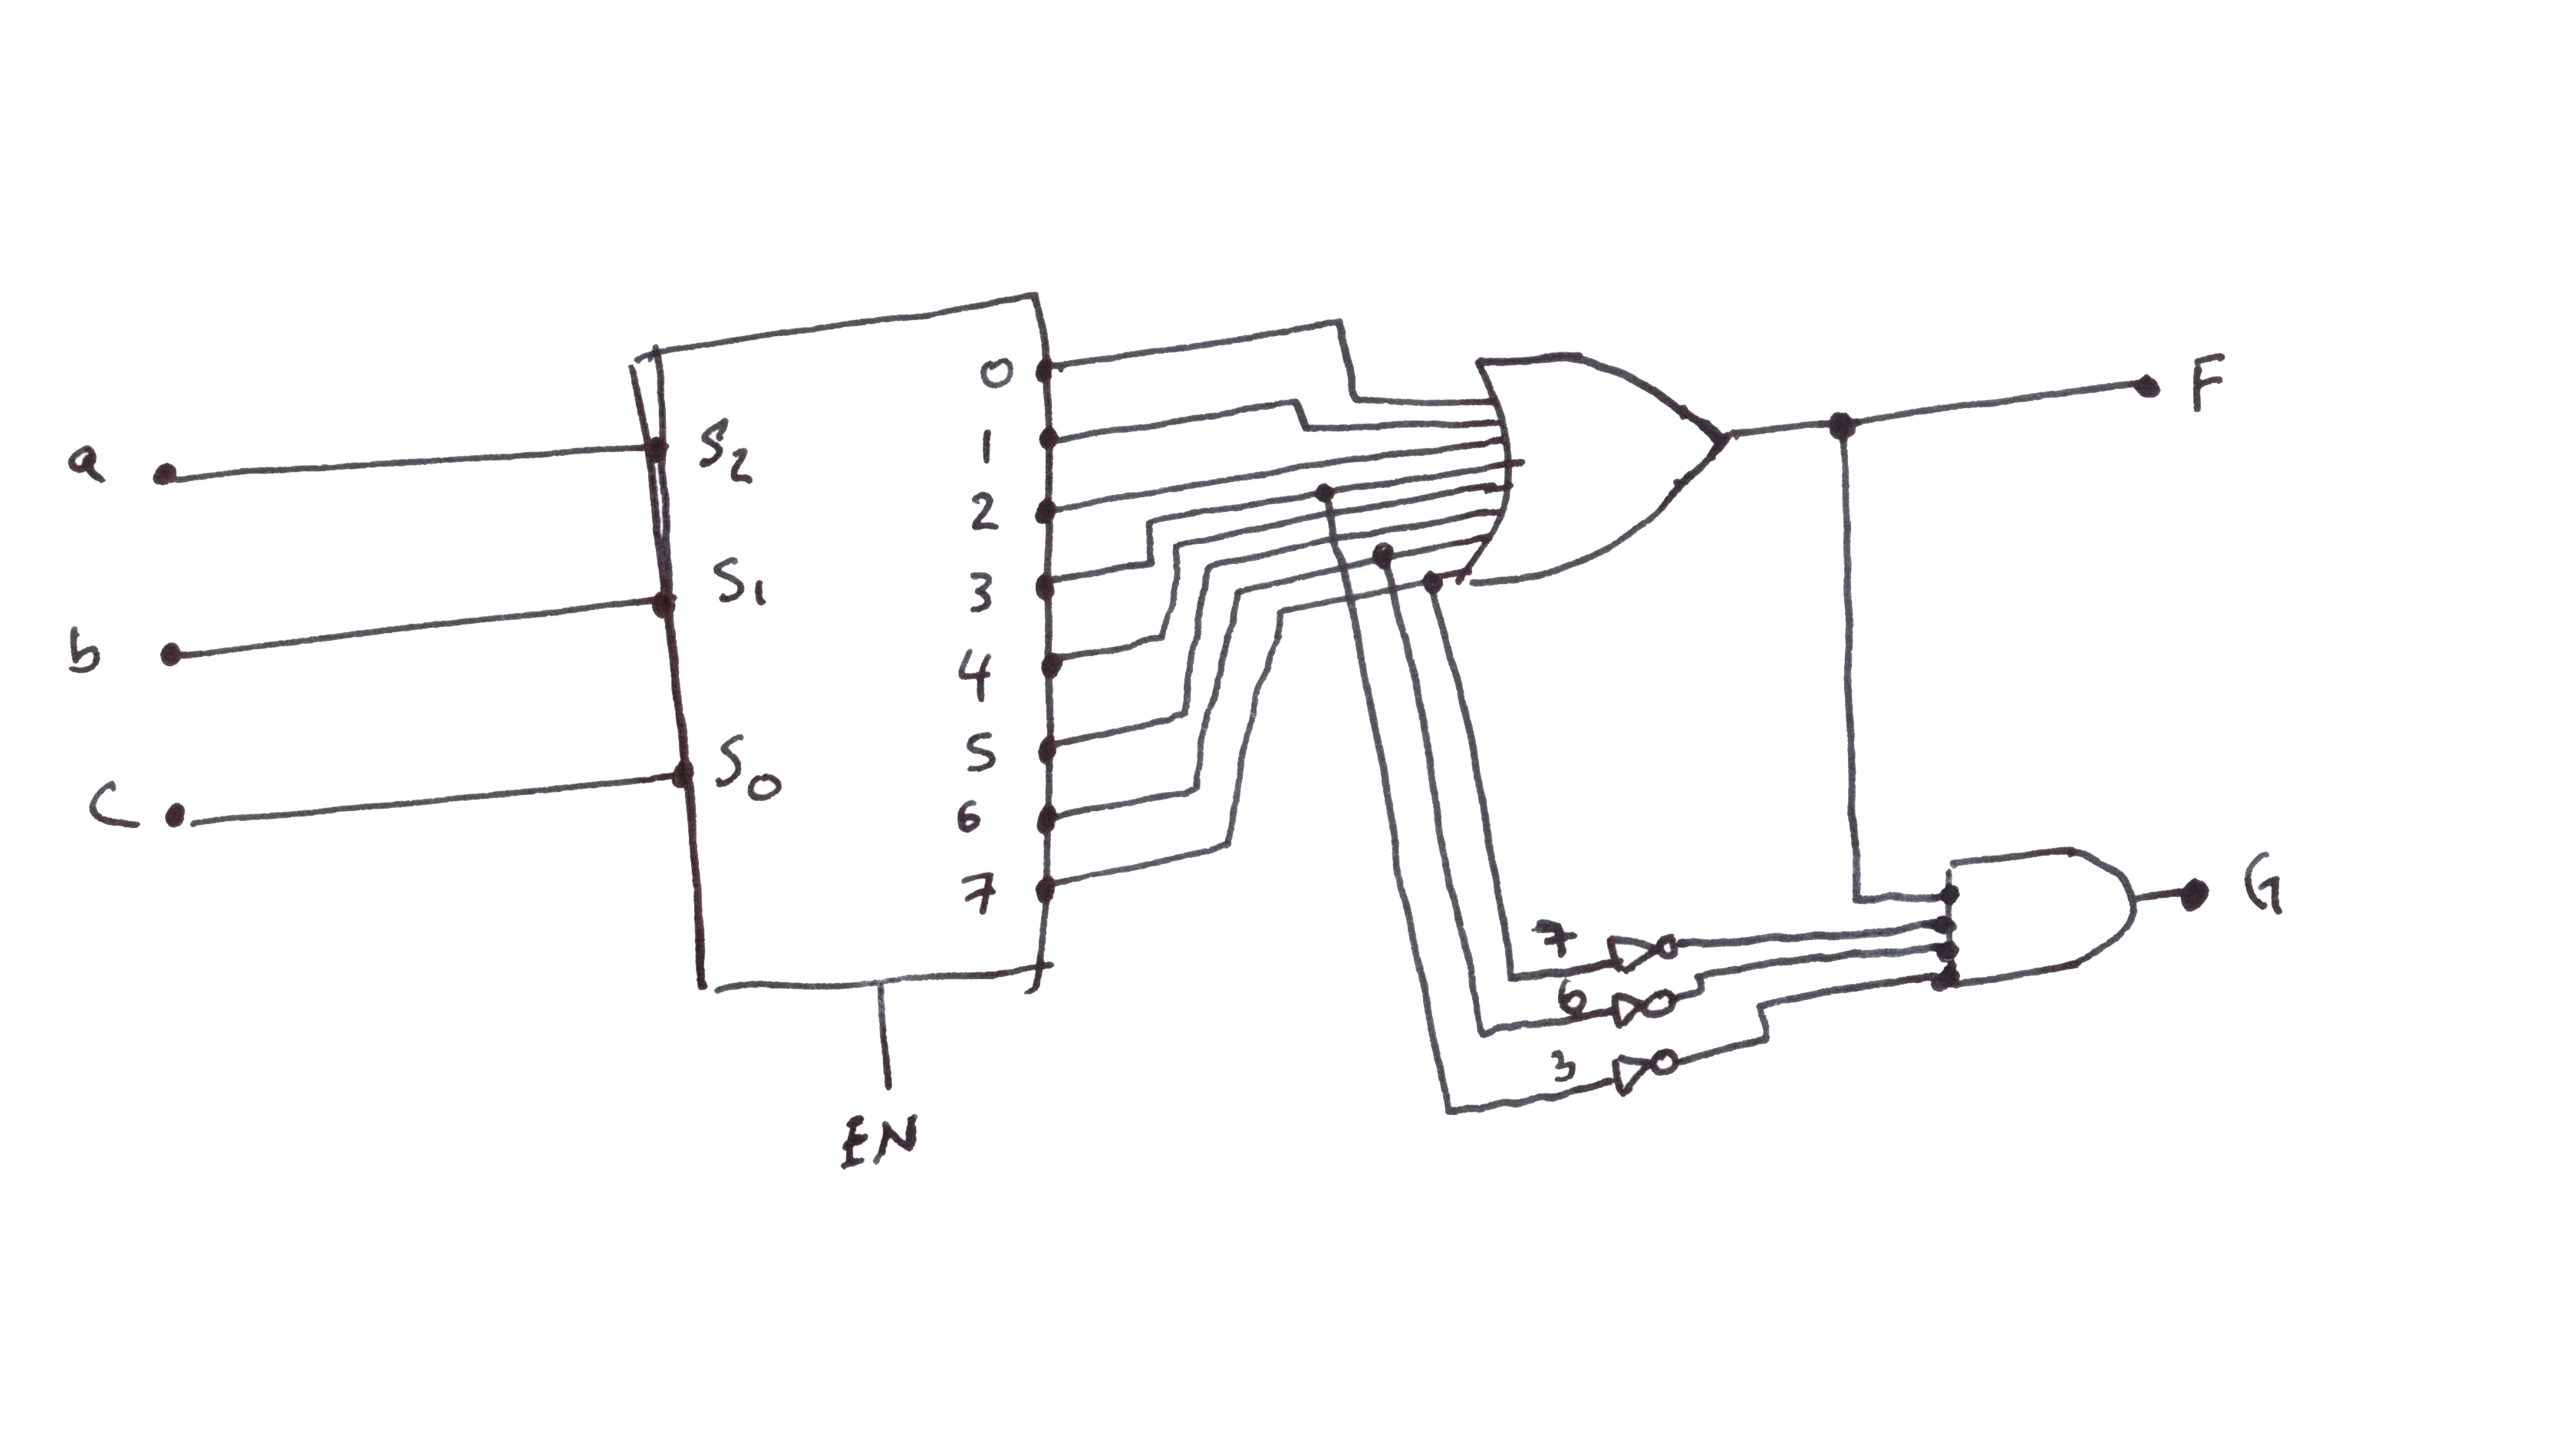
\includegraphics[width=\linewidth]{HW3_q2.png}
    \end{center}

    %###################################################################################

    \textbf{Problem 3:}

    \quad\quad (i)

    \begin{center}
        \begin{tabular} {cccc|c}
            w & x & y & z & P \\
            \hline
            0 & 0 & 0 & 0 & 0 \\
            0 & 0 & 0 & 1 & 0 \\
            0 & 0 & 1 & 0 & 0 \\
            0 & 0 & 1 & 1 & 0 \\
            0 & 1 & 0 & 0 & 0 \\
            0 & 1 & 0 & 1 & 0 \\
            0 & 1 & 1 & 0 & 1 \\
            0 & 1 & 1 & 1 & 1 \\
            1 & 0 & 0 & 0 & 1 \\
            1 & 0 & 0 & 1 & 1 \\
            1 & 0 & 1 & 0 & 1 \\
            1 & 0 & 1 & 1 & 1 \\
            1 & 1 & 0 & 0 & 1 \\
            1 & 1 & 0 & 1 & 1 \\
            1 & 1 & 1 & 0 & 1 \\
            1 & 1 & 1 & 1 & 1 \\
        \end{tabular}
    \end{center}

    \quad\quad (ii)

    \begin{center}
        \begin{tabular} {cc|cccc}
            & yz & &&& \\
            wx && 00 & 01 & 11 & 10 \\
            \hline
            & 00 & 0 & 0 & 0 & 0 \\
            & 01 & 0 & 0 & 1 & 1 \\
            & 11 & 1 & 1 & 1 & 1 \\
            & 10 & 1 & 1 & 1 & 1 \\
        \end{tabular}
    \end{center}

    \quad\quad 0000/0001/0011/0010 row - y and z changes 
    
    \quad\quad\quad\quad $=w+x$

    \quad\quad 0000/0001/0100/0101 square - x and z changes 
    
    \quad\quad\quad\quad $=w+y$

    \quad\quad\boxed{P(w,x,y,z)=(w+x)(w+y)}

    %###################################################################################

    \textbf{Problem 4:}

    % \begin{center}
    %     \begin{tabular} {cc|cccc}
    %         & de & &&& \\
    %         bc && 00 & 01 & 11 & 10 \\
    %         \hline
    %         & 00 & 0 & 1 & 3 & 2 \\
    %         & 01 & 4 & 5 & 7 & 6 \\
    %         & 11 & 12 & 13 & 15 & 14 \\
    %         & 10 & 8 & 9 & 11 & 10 \\
    %     \end{tabular}
    % \end{center}

    % \begin{center}
    %     \begin{tabular} {cc|cccc}
    %         & de & &&& \\
    %         bc && 00 & 01 & 11 & 10 \\
    %         \hline
    %         & 00 & 16 & 17 & 19 & 18 \\
    %         & 01 & 20 & 21 & 23 & 22 \\
    %         & 11 & 28 & 29 & 31 & 30 \\
    %         & 10 & 24 & 25 & 27 & 26 \\
    %     \end{tabular}
    % \end{center}

    \begin{center}
        a=0
        \begin{tabular} {cc|cccc}
            & de & &&& \\
            bc && 00 & 01 & 11 & 10 \\
            \hline
            & 00 & 0 & 0 & 0 & 1 \\
            & 01 & 1 & 0 & 1 & 0 \\
            & 11 & 1 & 0 & 1 & 0 \\
            & 10 & 1 & 1 & 0 & 1 \\
        \end{tabular}
        \quad\quad
        a=1
        \begin{tabular} {cc|cccc}
            & de & &&& \\
            bc && 00 & 01 & 11 & 10 \\
            \hline
            & 00 & 0 & 0 & 0 & 1 \\
            & 01 & 1 & 1 & 1 & 1 \\
            & 11 & 0 & 1 & 1 & 0 \\
            & 10 & 1 & 1 & 0 & 1 \\
        \end{tabular}
    \end{center}

    00100/01100 pair - b changes; occurs only when a = 0

    \quad\quad $= a'cd'e'$

    01000/01001 pair and 11000/11001 pair - e and a changes

    \quad\quad $= bc'd'$

    00111/01111 pair and 10111/11111 - b and a changes

    \quad\quad $=cde$

    00010/01010 pair and 10010/11010 pair - b and a changes

    \quad\quad $= c'de'$

    10101/10111/11101/11111 square - b and d changes

    \quad\quad $= ace$

    10100/10101/10111/10110 row - d and e changes

    \quad\quad $=ab'c$

    \boxed{Z(a,b,c,d,e)=a'cd'e'+bc'd'+cde+c'de'+ace+ab'c}

    %###################################################################################

    \textbf{Problem 5:}

    \begin{center}
        \begin{tabular} {cc|ccc|ccccccccc|cccc}
            &b&&& &&& &&& &&& &&& \\
            a&&&& 0&&& &&& &&&1 &&& \\

            \hline

            &&&&&&&&&&&&&&&&& \\
            &&&& ef & &&&&                    &&&& de & &&& \\
            &&&cd && 00 & 01 & 11 & 10 &&     &&bc && 00 & 01 & 11 & 10 \\
            \hline
            &&&& 00 & x & 0 & 1 & 0 &&&       && 00 & x & 0 & 1 & 0 \\
            &0&&& 01 & 1 & 1 & 0 & 1 &&&      && 01 & 1 & 0 & 0 & 1 \\
            &&&& 11 & 1 & 1 & x & 0 &&&      && 11 & 1 & 0 & 1 & 0 \\
            &&&& 10 & 0 & 0 & 0 & 0 &&&       && 10 & 0 & 1 & x & x \\
            &&&&&&&&&&&&&&&&& \\

            &&&&&&&&&&&&&&&&& \\
            &&&& ef & &&&&                    &&&& de & &&& \\
            &&&cd && 00 & 01 & 11 & 10 &&     &&bc && 00 & 01 & 11 & 10 \\
            \hline
            &&&& 00 & 0 & 0 & x & x &&&       && 00 & 1 & 1 & 0 & 1 \\
            &0&&& 01 & x & 1 & 1 & 1 &&&      && 01 & x & 0 & 0 & 1 \\
            &&&& 11 & 0 & 0 & 0 & 1 &&&       && 11 & 0 & 0 & 0 & 0 \\
            &&&& 10 & 0 & 0 & x & 1 &&&       && 10 & 1 & x & 1 & x \\
            &&&&&&&&&&&&&&&&& \\
        \end{tabular}
    \end{center}

    000100/000101/001100/001101 square - c and f changes

    \quad\quad $=a'b'de'$

    000011 point and 010011 point - b changes

    \quad\quad $=ac'd'ef$

    000100/000110 pair and 100100/100110 - e and a changes

    \quad\quad $=b'c'df'$

    010100/011100 pair and 000100/001100- c and b changes

    \quad\quad $=a'de'f'$

    011011/011111 pair - d changes

    \quad\quad $=a'bcef$

    011001/101011 pair and 111001/111011 pair - a and e changes

    \quad\quad $=bcd'f$

    100100/100101/100111/100110 row - e and f changes

    \quad\quad $=ab'c'd$

    100010/100110/101110/101010 column - c and d changes

    \quad\quad $=ab'ef'$

    110000/110001/111000/111001 square - c and f changes

    \quad\quad $abd'e'$

    110000/110100/110010/110110 square - e and d changes

    \quad\quad $abc'f'$

    \fbox{%
        \parbox{0.95\textwidth}{%
            $Y(a,b,c,d,e,f)=a'b'de'+ac'd'ef+b'c'df'+a'de'f'+a'bcef+ \\
            bcd'f+ab'c'd+ab'ef'+abd'e'+abc'f'$
        }%
    }

    %###################################################################################

    \textbf{Problem 6:}

    \begin{center}
        \begin{tabular} {c}
              \\
            0 \\
              \\
            1 \\
              \\
            2 \\
              \\
            3 \\
              \\
            4 \\
              \\
            5 \\
              \\
            6 \\
              \\
            7 
        \end{tabular}
        \begin{tabular} {cccc|c}
            a & b & c & d & g \\
            \hline
            0 & 0 & 0 & 0 & 0 \\
            0 & 0 & 0 & 1 & 1 \\
            \hdashline
            0 & 0 & 1 & 0 & 1 \\
            0 & 0 & 1 & 1 & 1 \\
            \hdashline
            0 & 1 & 0 & 0 & 0 \\
            0 & 1 & 0 & 1 & 1 \\
            \hdashline
            0 & 1 & 1 & 0 & 0 \\
            0 & 1 & 1 & 1 & 0 \\
            \hdashline
            1 & 0 & 0 & 0 & 0 \\
            1 & 0 & 0 & 1 & 1 \\
            \hdashline
            1 & 0 & 1 & 0 & 0 \\
            1 & 0 & 1 & 1 & 0 \\
            \hdashline
            1 & 1 & 0 & 0 & 0 \\
            1 & 1 & 0 & 1 & 1 \\
            \hdashline
            1 & 1 & 1 & 0 & 1 \\
            1 & 1 & 1 & 1 & 1 \\
        \end{tabular}
        \begin{tabular} {c}
            \\
          = d \\
            \\
          = 1 \\
            \\
          = d \\
            \\
          = 0 \\
            \\
          = d \\
            \\
          = 0 \\
            \\
          = d \\
            \\
          = 1 
      \end{tabular}
    \end{center}

    \begin{center}
        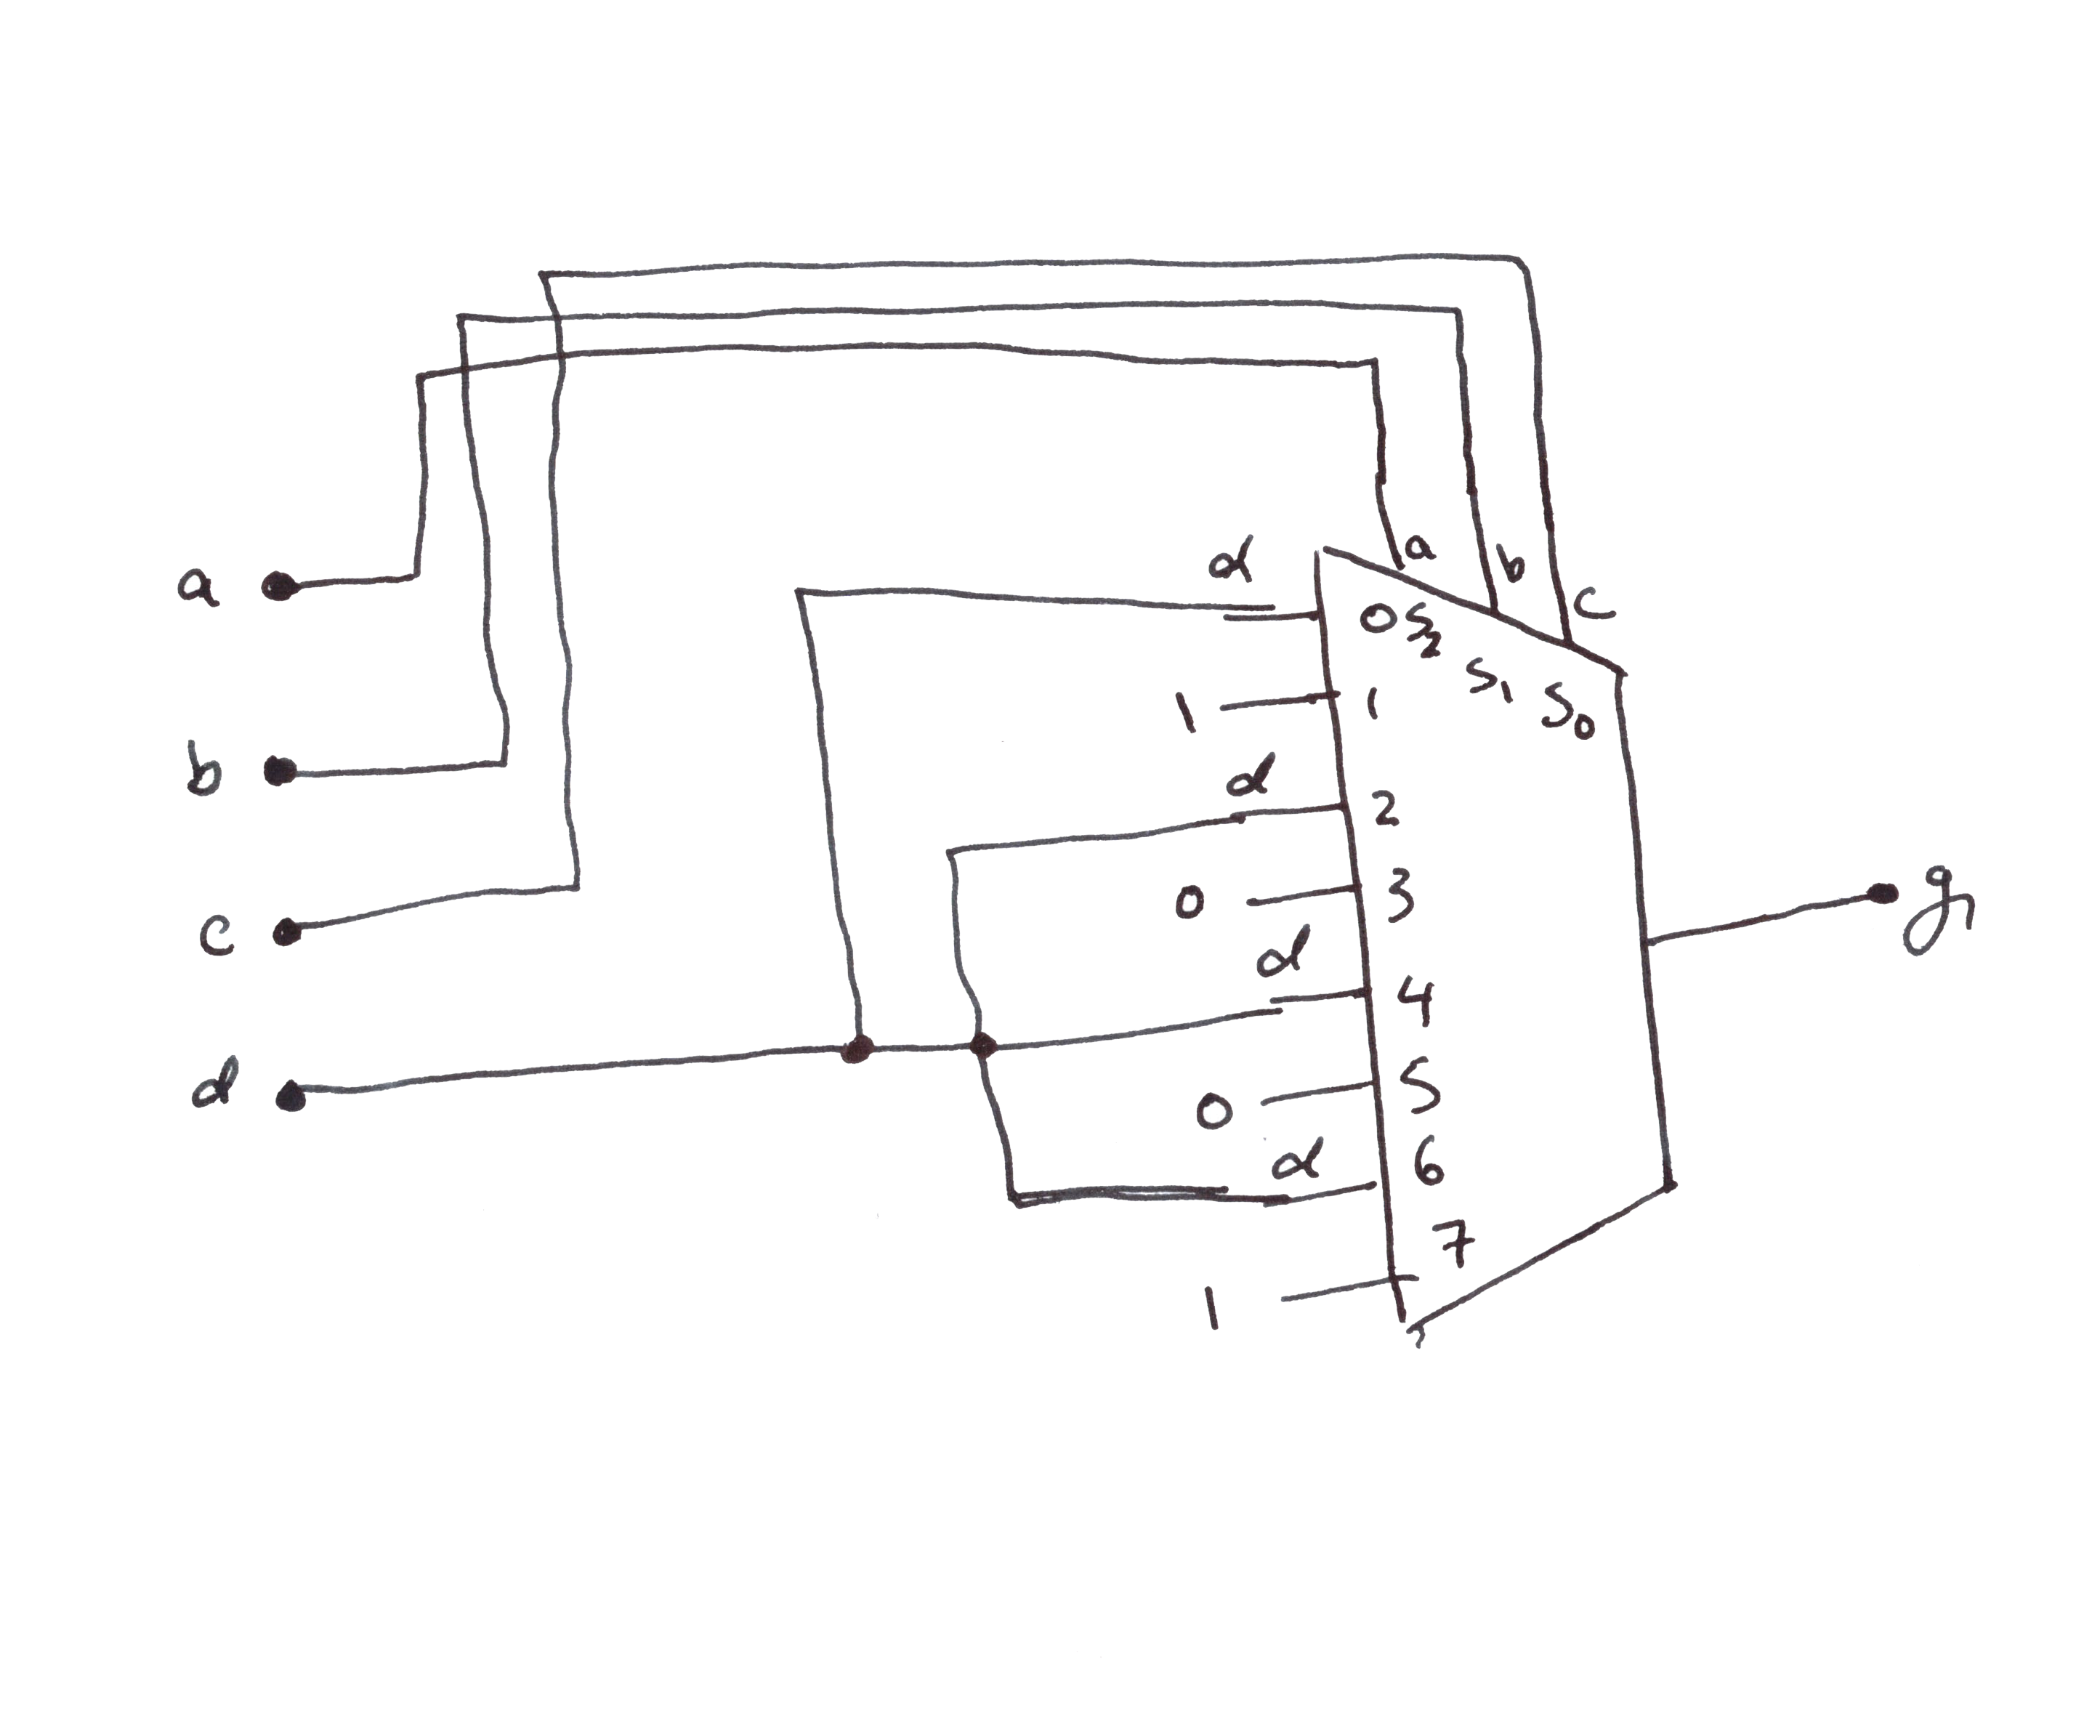
\includegraphics[width=\linewidth]{HW3_q6.png}
    \end{center}

    %###################################################################################

    \textbf{Problem 7:}

    \begin{center}
        \begin{tabular} {cccc|c}
            w & x & y & z & f \\
            \hline
            0 & 0 & 0 & 0 & 0 \\
            0 & 0 & 0 & 1 & 1 \\
            0 & 0 & 1 & 0 & 0 \\
            0 & 0 & 1 & 1 & 0 \\
            0 & 1 & 0 & 0 & 0 \\
            0 & 1 & 0 & 1 & 1 \\
            0 & 1 & 1 & 0 & 0 \\
            0 & 1 & 1 & 1 & 0 \\
            1 & 0 & 0 & 0 & 1 \\
            1 & 0 & 0 & 1 & 1 \\
            1 & 0 & 1 & 0 & 1 \\
            1 & 0 & 1 & 1 & 1 \\
            1 & 1 & 0 & 0 & 0 \\
            1 & 1 & 0 & 1 & 1 \\
            1 & 1 & 1 & 0 & 0 \\
            1 & 1 & 1 & 1 & 0 \\
        \end{tabular}
        \quad\quad\quad
        \begin{tabular} {cccc|c}
            w & x & y & z & g \\
            \hline
            0 & 0 & 0 & 0 & 0 \\
            0 & 0 & 0 & 1 & 1 \\
            0 & 0 & 1 & 0 & 0 \\
            0 & 0 & 1 & 1 & 1 \\
            0 & 1 & 0 & 0 & 0 \\
            0 & 1 & 0 & 1 & 0 \\
            0 & 1 & 1 & 0 & 0 \\
            0 & 1 & 1 & 1 & 1 \\
            1 & 0 & 0 & 0 & 1 \\
            1 & 0 & 0 & 1 & 1 \\
            1 & 0 & 1 & 0 & 0 \\
            1 & 0 & 1 & 1 & 1 \\
            1 & 1 & 0 & 0 & 1 \\
            1 & 1 & 0 & 1 & 0 \\
            1 & 1 & 1 & 0 & 0 \\
            1 & 1 & 1 & 1 & 1 \\
        \end{tabular}
    \end{center}

    \quad\quad (i)

    \begin{center}
        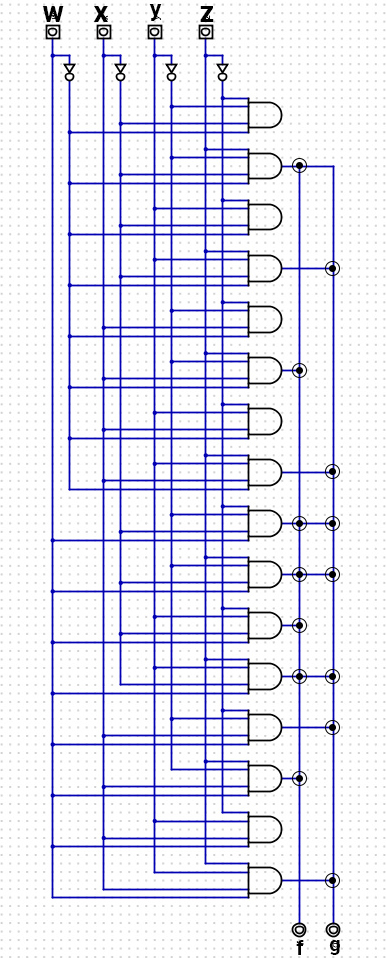
\includegraphics[width=50mm,scale=0.5]{HW3_q7.jpg}
    \end{center}

    \quad\quad (ii)

    \begin{center}
        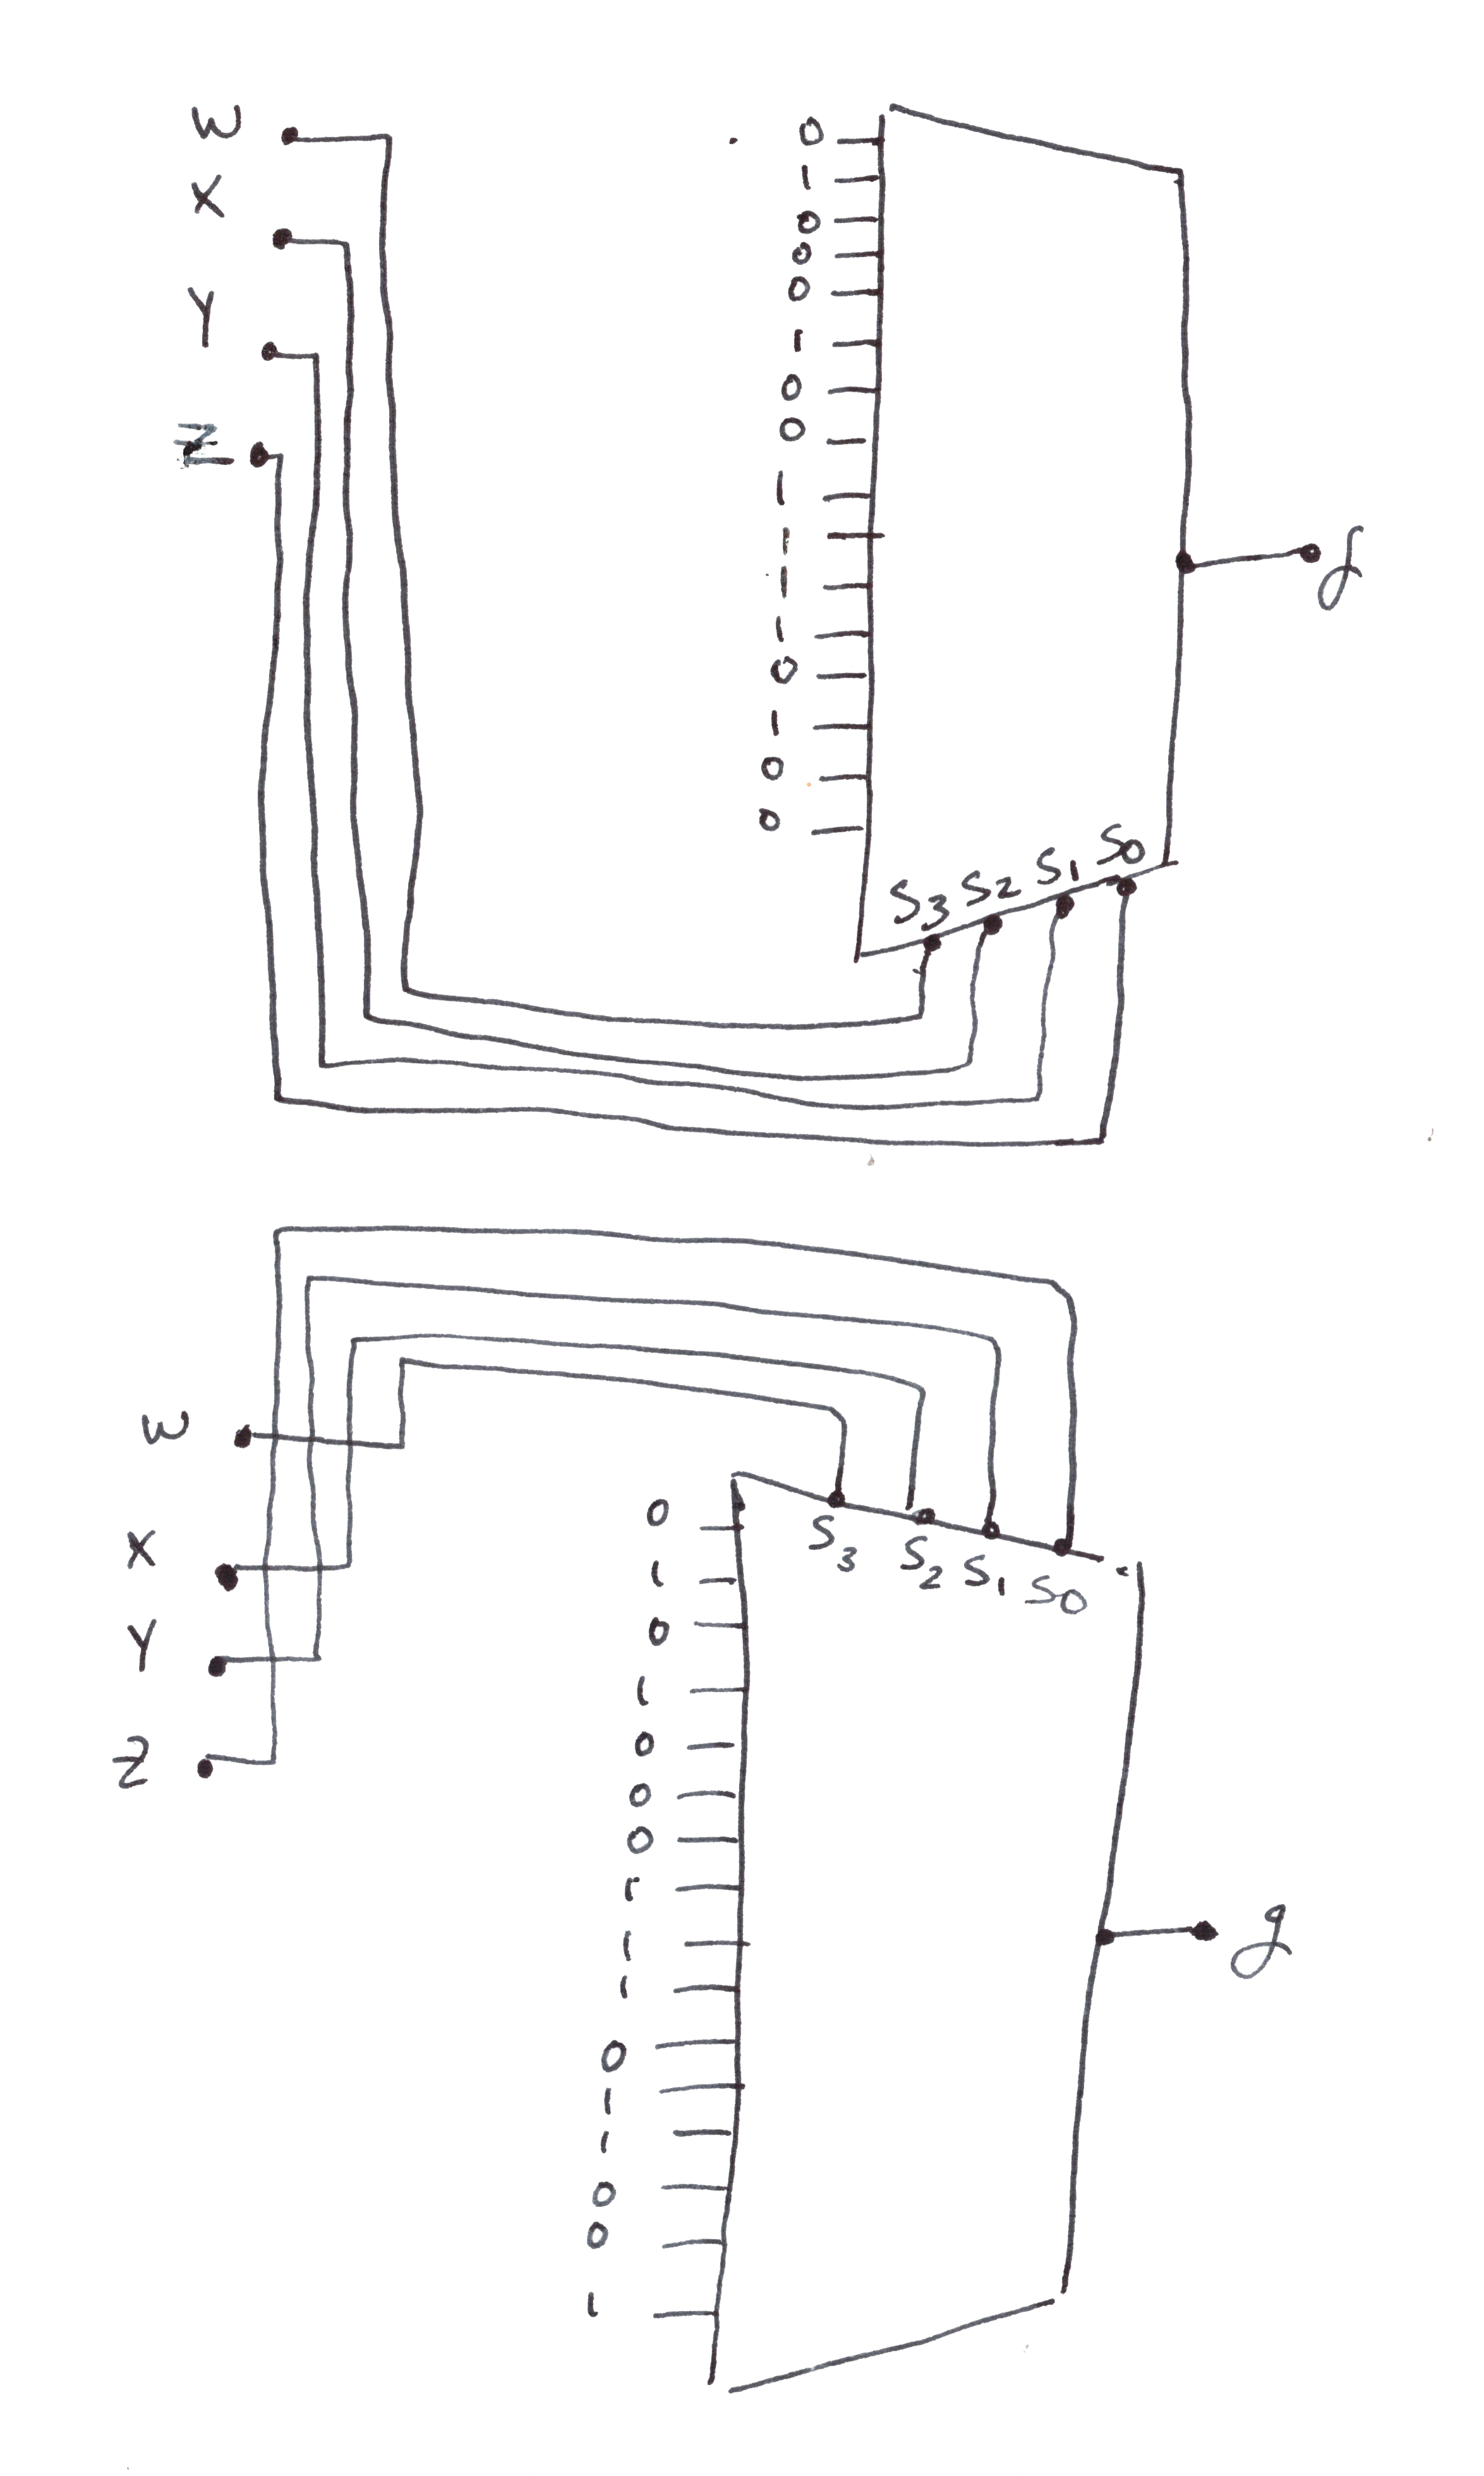
\includegraphics[width=\linewidth]{HW3_q7.2.png}
    \end{center}

    \quad\quad (iii)

    \begin{center}
        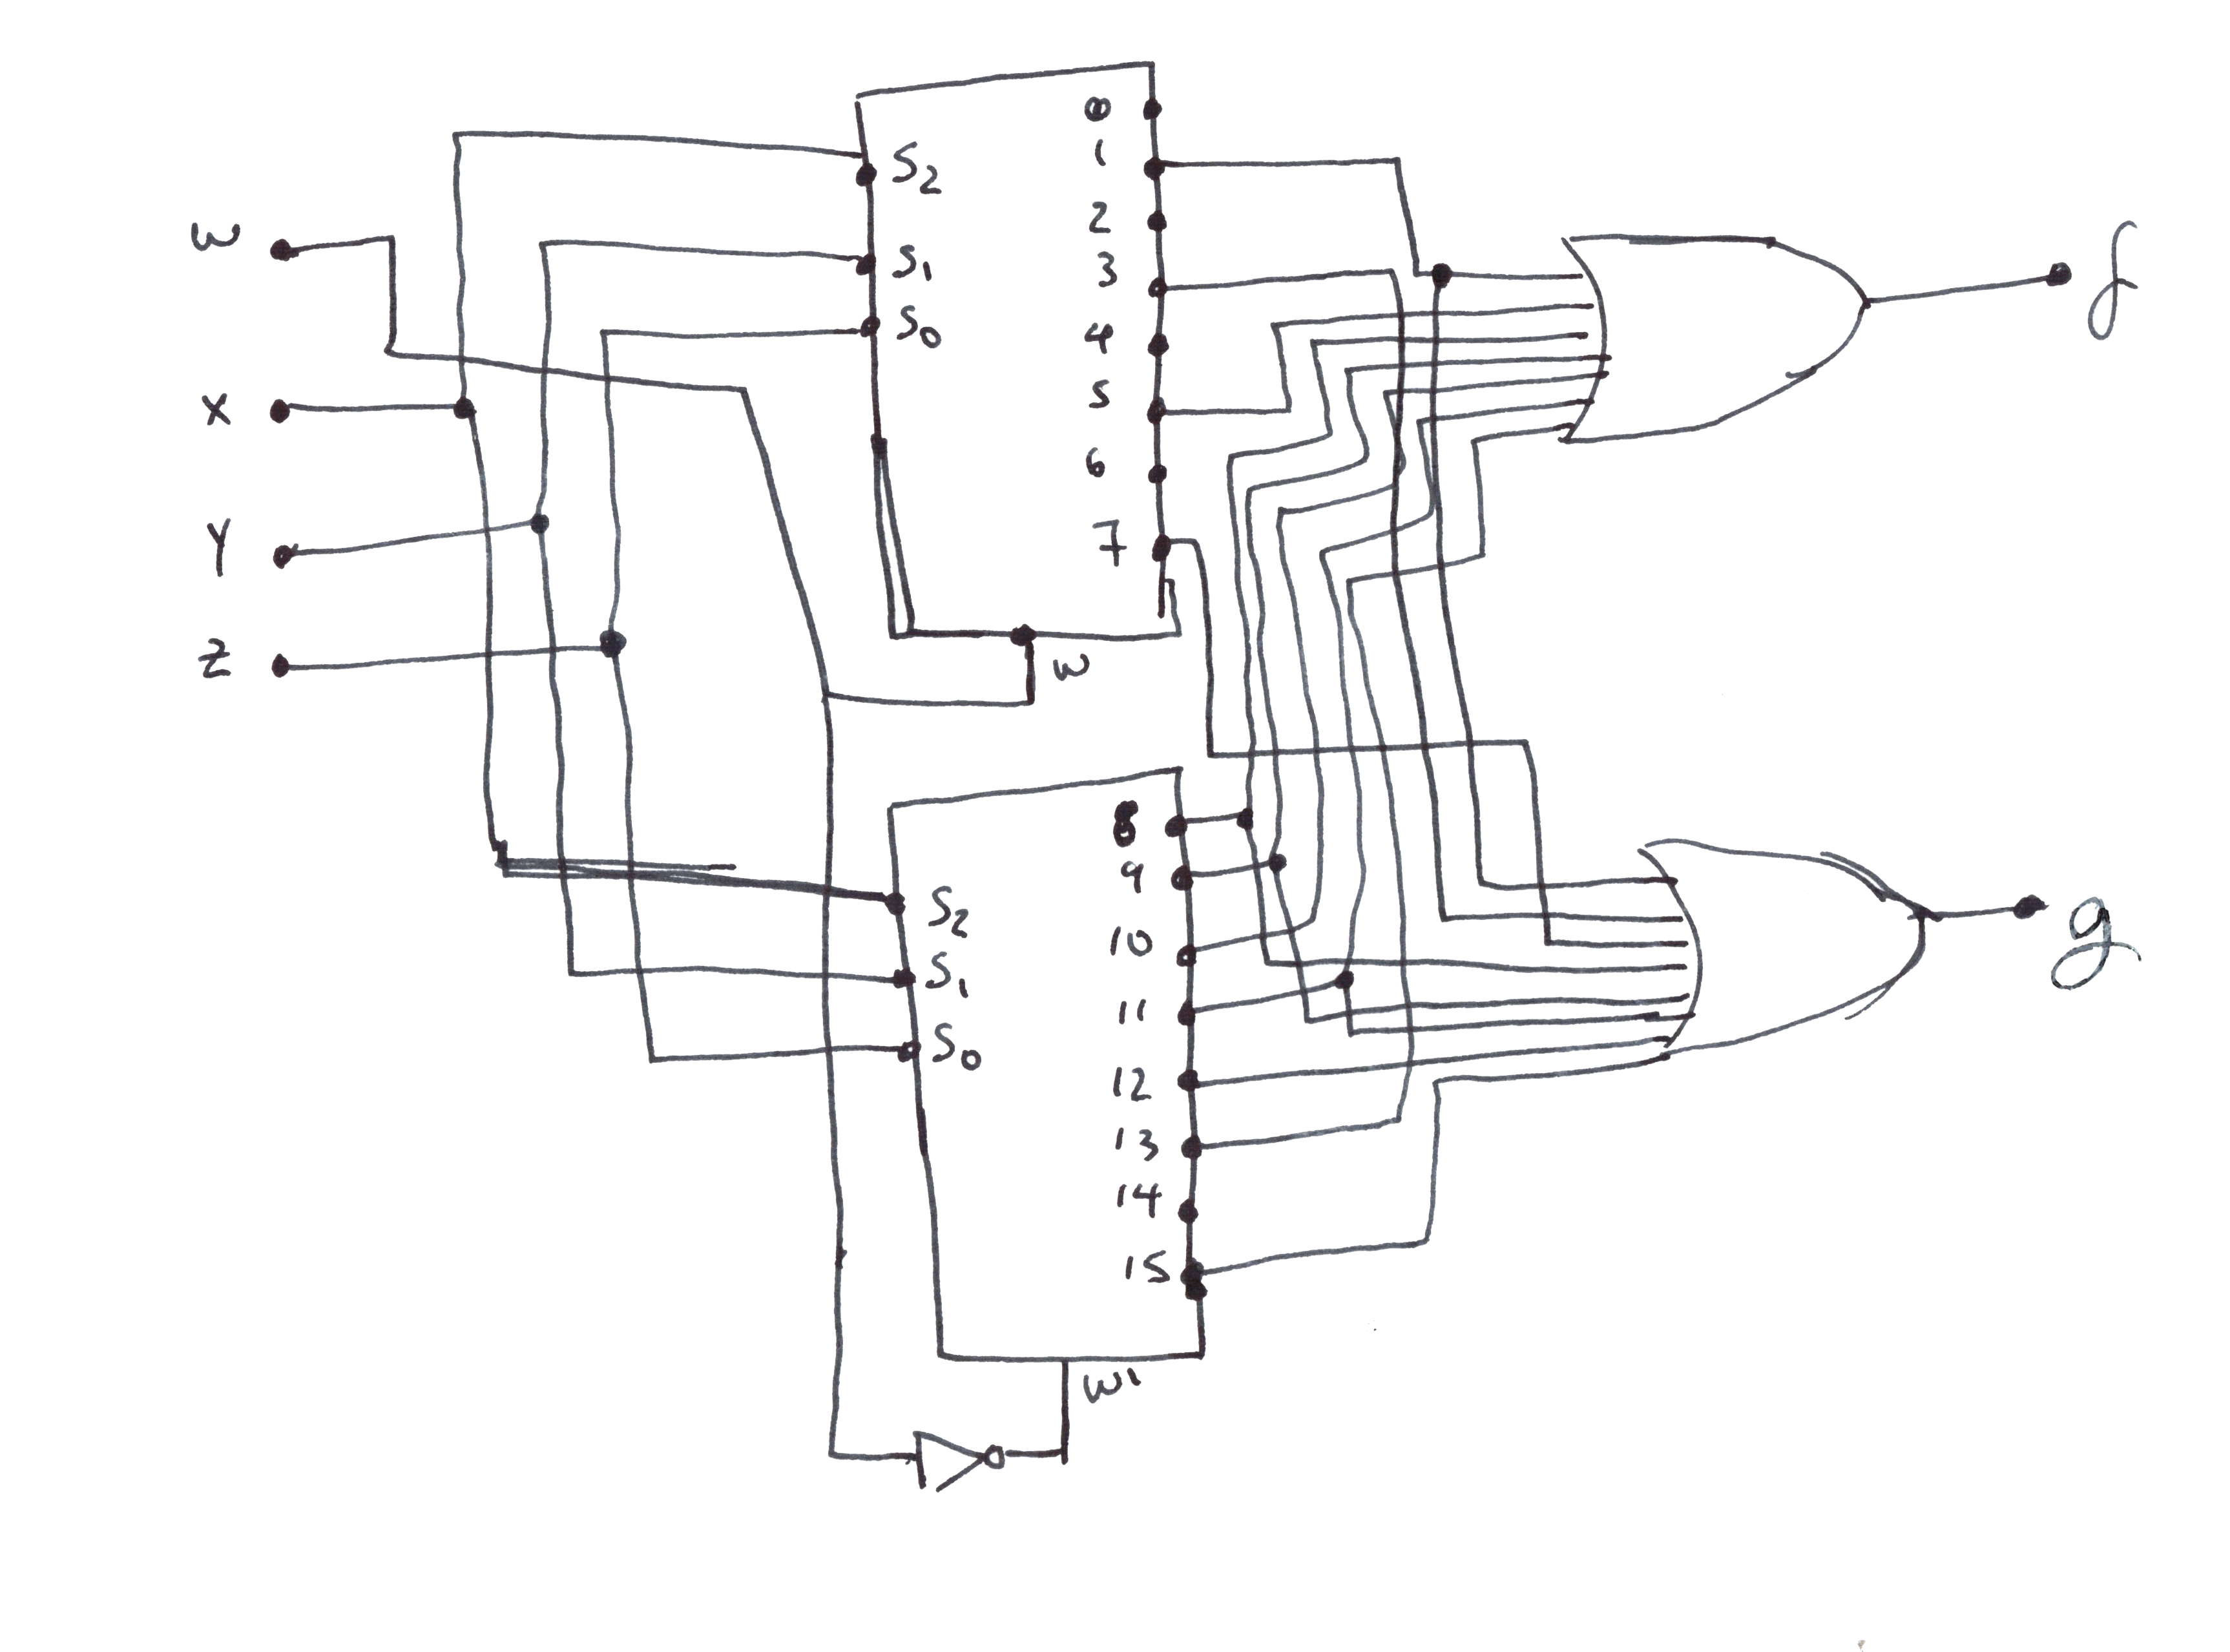
\includegraphics[width=\linewidth]{HW3_q7.3.png}
    \end{center}

    %###################################################################################

    \textbf{Problem 8:}

    \quad\quad (i)

    \begin{center}
        \begin{tabular} {ccc|c}
            a & b & c & g \\
            \hline
            0 & 0 & 0 & 1 \\
            0 & 0 & 1 & 1 \\
            0 & 1 & 0 & 0 \\
            0 & 1 & 1 & 0 \\
            1 & 0 & 0 & 0 \\
            1 & 0 & 1 & 0 \\
            1 & 1 & 0 & 1 \\
            1 & 1 & 1 & 1 \\
        \end{tabular}
    \end{center}

    \quad\quad (ii)

    \quad\quad\quad\quad\boxed{g(a,b,c) = (ab'c)+(ab'c')+(a'bc)+(a'bc')}

    \quad\quad (iii)

    \begin{center}
        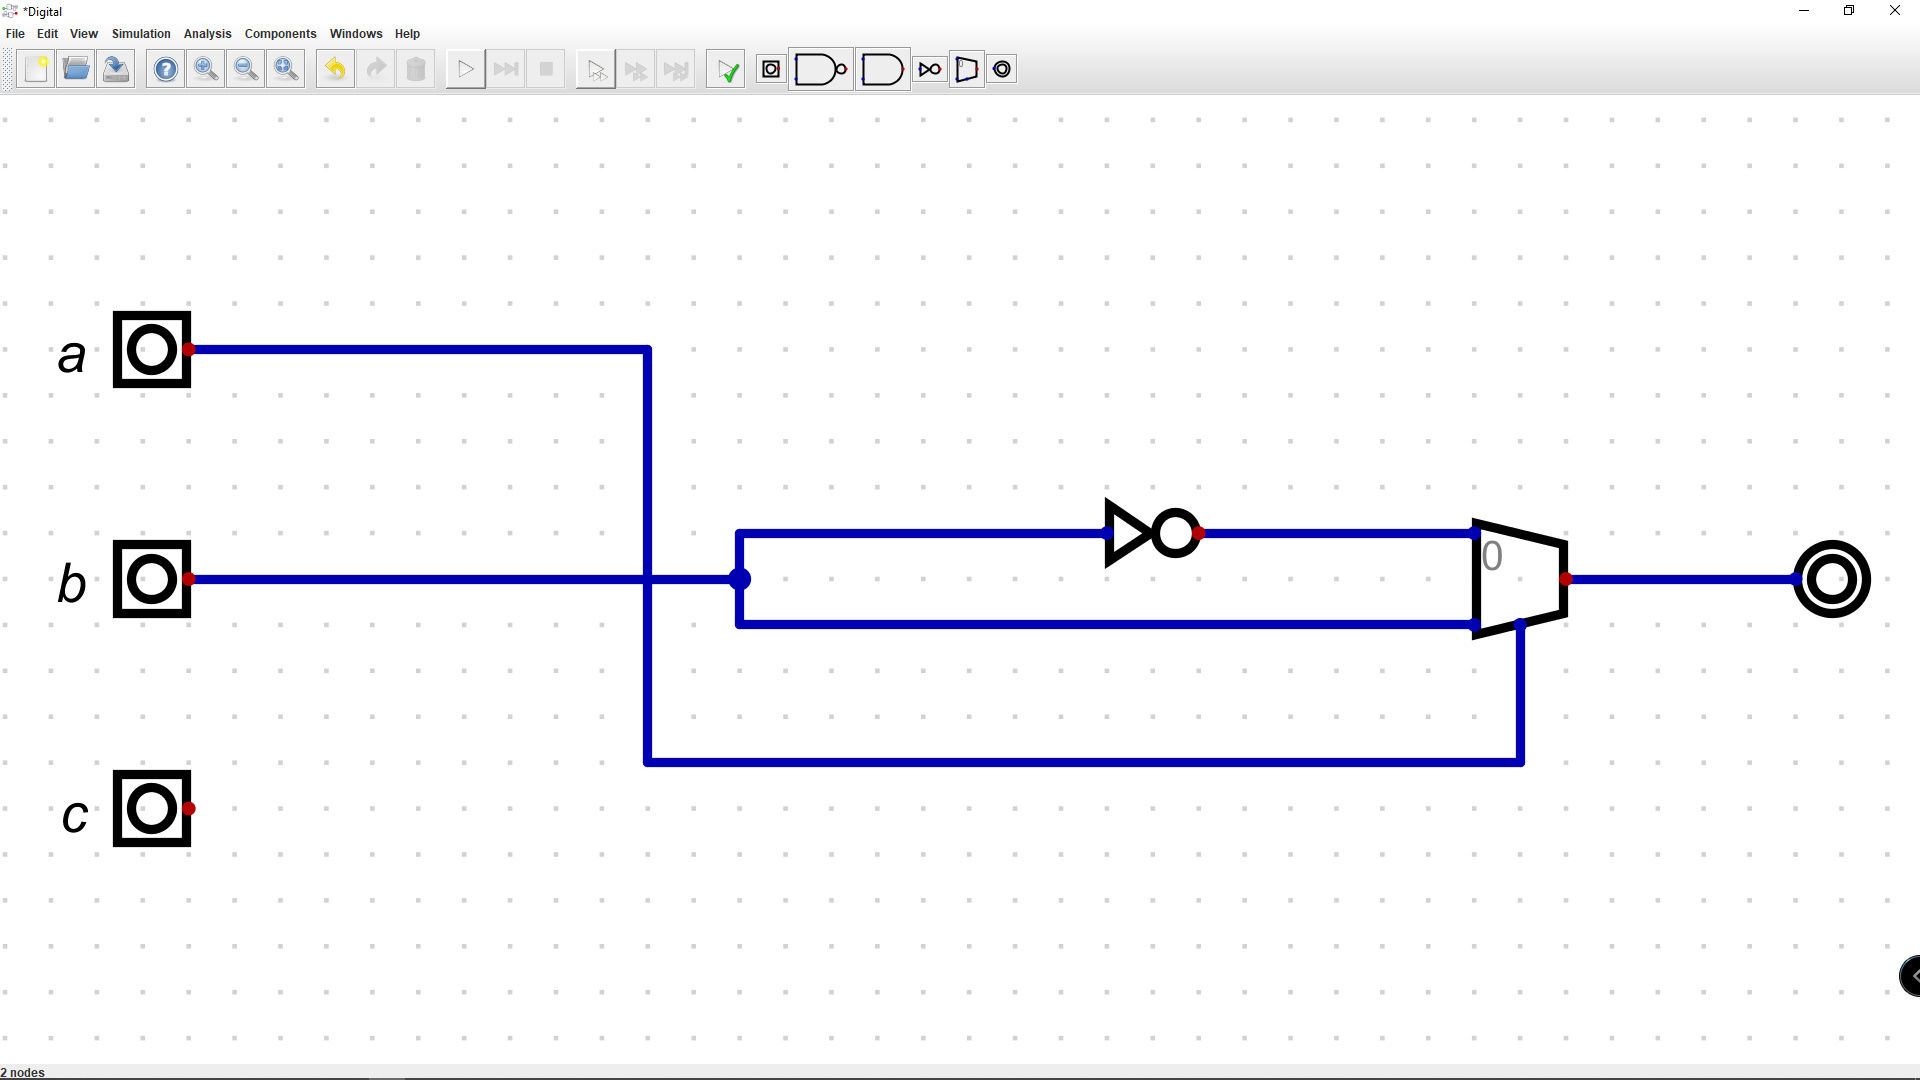
\includegraphics[width=\linewidth]{HW3_q8.jpg}
    \end{center}

    %###################################################################################

    \textbf{Problem 9:}

    \begin{center}
        \begin{tabular} {ccc|c}
            a & b & c & X \\
            \hline
            0 & 0 & 0 & 0 \\
            0 & 0 & 1 & 1 \\
            0 & 1 & 0 & 1 \\
            0 & 1 & 1 & 1 \\
            1 & 0 & 0 & 1 \\
            1 & 0 & 1 & 0 \\
            1 & 1 & 0 & 1 \\
            1 & 1 & 1 & 1 \\
        \end{tabular}
        \quad\quad
        \begin{tabular} {ccc|c}
            a & b & c & Y \\
            \hline
            0 & 0 & 0 & 1 \\
            0 & 0 & 1 & 1 \\
            0 & 1 & 0 & 1 \\
            0 & 1 & 1 & 1 \\
            1 & 0 & 0 & 0 \\
            1 & 0 & 1 & 1 \\
            1 & 1 & 0 & 0 \\
            1 & 1 & 1 & 1 \\
        \end{tabular}
        \quad\quad
        \begin{tabular} {ccc|c}
            a & b & c & Z \\
            \hline
            0 & 0 & 0 & x \\
            0 & 0 & 1 & x \\
            0 & 1 & 0 & x \\
            0 & 1 & 1 & 1 \\
            1 & 0 & 0 & 1 \\
            1 & 0 & 1 & 0 \\
            1 & 1 & 0 & 1 \\
            1 & 1 & 1 & 1 \\
        \end{tabular}
    \end{center}

    \quad\quad (i)

    \begin{center}
        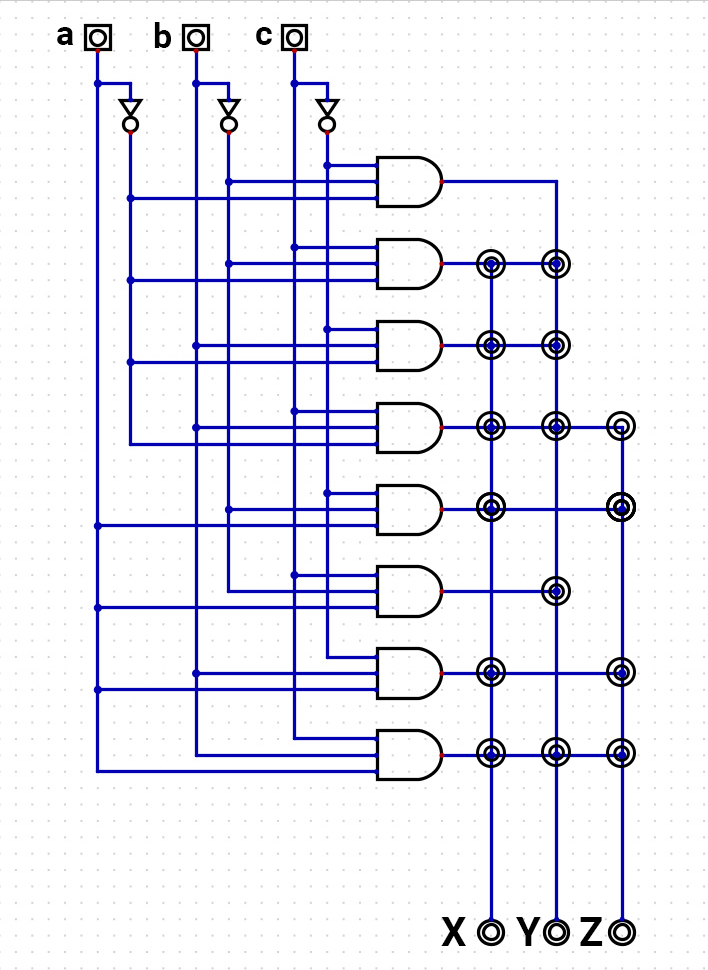
\includegraphics[width=70mm]{HW3_q9.jpg}
    \end{center}

    \quad\quad (ii)

    \begin{center}
        \begin{tabular} {cc|cccc}
            & bc & &&& \\
            a && 00 & 01 & 11 & 10 \\
            \hline
            & 0 & 0 & 1 & 1 & 1 \\
            & 1 & 1 & 0 & 1 & 1 \\
        \end{tabular}
    \end{center}

    001/011 pair - b changes

    \quad\quad $=a'c$

    100/110 pair - b changes 

    \quad\quad $=ac'$

    011/010/111/110 square - a and c changes

    \quad\quad $=b$

    \boxed{X(a,b,c)=a'c+ac'+b}

    \begin{center}
        \begin{tabular} {cc|cccc}
            & bc & &&& \\
            a && 00 & 01 & 11 & 10 \\
            \hline
            & 0 & 1 & 1 & 1 & 1 \\
            & 1 & 0 & 1 & 1 & 0 \\
        \end{tabular}
    \end{center}

    000/001/011/010 row - b and c changes

    \quad\quad $=a'$

    101/111 pair - b changes

    \quad\quad $=ac$

    \boxed{Y(a,b,c)=a'+ac}

    \begin{center}
        \begin{tabular} {cc|cccc}
            & bc & &&& \\
            a && 00 & 01 & 11 & 10 \\
            \hline
            & 0 & x & x & 1 & x \\
            & 1 & 1 & 0 & 1 & 1 \\
        \end{tabular}
    \end{center}

    000/100/010/110 square - a and b changes

    \quad\quad $=c'$

    011/010/111/110 square - a and c changes

    \quad\quad $=b$

    \boxed{Z(a,b,c)=c'+b}

    \begin{center}
        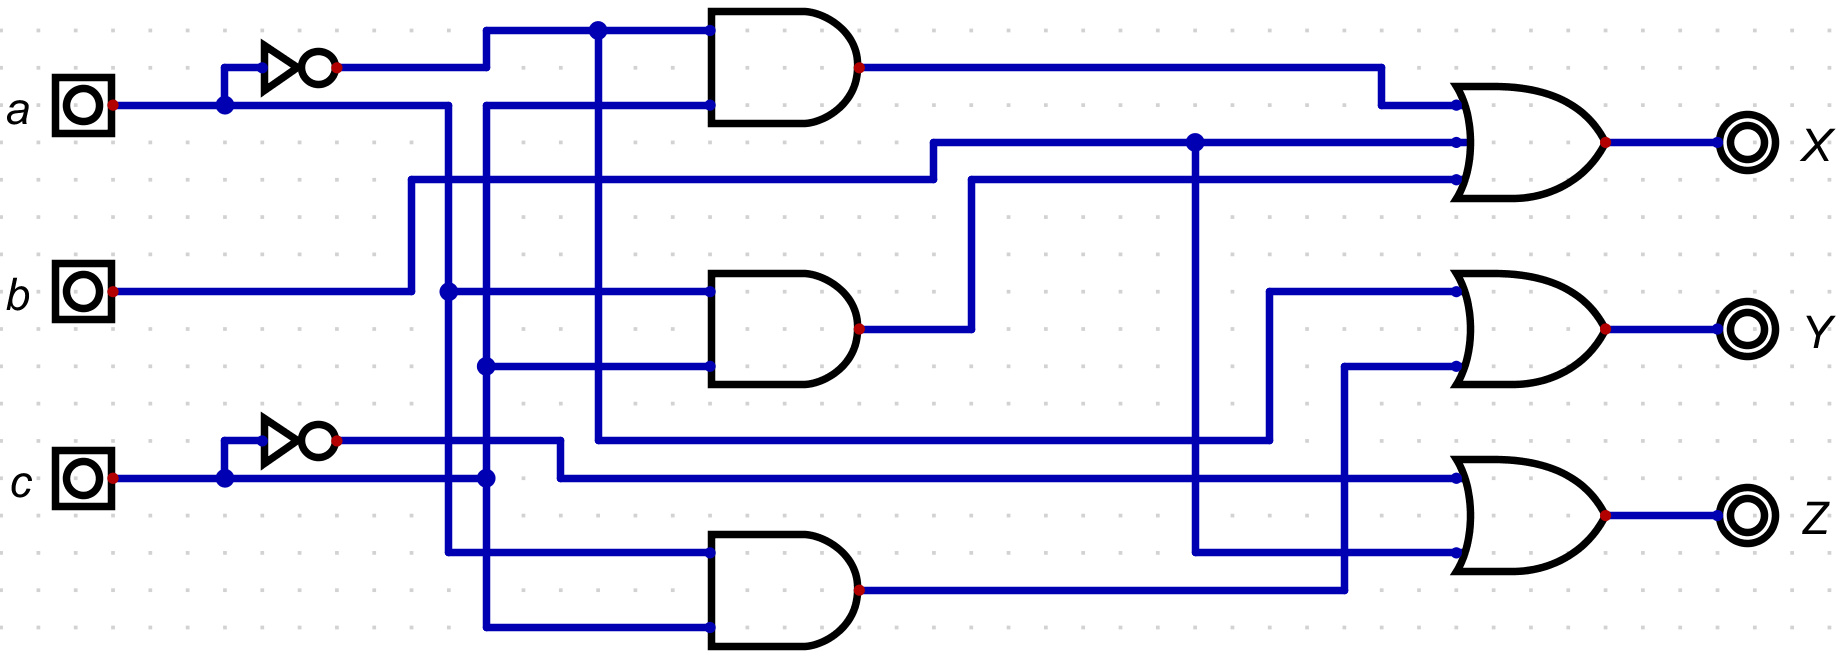
\includegraphics[width=\linewidth]{HW3_q9.1.jpg}
    \end{center}

\end{document}